%- block legend
Pete tem uma pequena fazenda onde ele cultiva e colhe batatas.

A fazendinha de Pete é descrita como uma matriz de $N$ linhas e $M$ colunas.
Na posição $(i,j)$ da fazenda ($1 \leq i \leq N, 1 \leq j \leq M$) existem $B_{i,j}$ batatas maduras, prontas para a colheita.

Pete tem uma colheitadeira mágica, que pode ser acionada uma única vez. Ao
acionar a colheitadeira em uma posição $(l,c)$ e configurá-la para uma distância
não negativa $D$, serão colhidas, de uma só vez, todas as batatas
em todas as posições $(i,j)$ tais que $|i-l| + |j-c| \leq D$.

Pete precisa colher pelo menos $T$ batatas ao todo. Pete pode acionar a
colheitadeira na posição que quiser, mas, para economizar com os gastos de seu
uso, precisa configurá-la com a menor distância $D$ possível.

Qual é a menor distância $D$ necessária para configurar a colheitadeira de forma
que pelo menos $T$ batatas sejam colhidas?
%- endblock

%- block input
A primeira linha contém três inteiros $N$, $M$ e $T$
($\VAR{N.min} \leq N, M \leq \VAR{M.max}$,
 $\VAR{T.min} \leq T \leq \VAR{T.max | sci}$), o número de linhas e de colunas da
fazenda, e o número mínimo de batatas a serem colhidas.

As próximas $N$ linhas contém $M$ inteiros $B_{i,j}$ cada
($\VAR{B.min} \leq B_{i,j} \leq \VAR{B.max}$), indicando o número de batatas em
cada posição da fazenda.
%- endblock

%- block output
Se não for possível colher pelo menos $T$ batatas, imprima \texttt{-1}.

Caso contrário, imprima o menor valor de $D$ necessário para se colher pelo menos
$T$ batatas.
\newpage % pro exemplo ficar na outra pagina, junto com a figura

%- endblock

%- block explanation_0
A figura abaixo apresenta o primeiro exemplo de entrada. Ao acionar a
colheitadeira na posição $(2,1)$, com $D=2$, Pete consegue colher 74 batatas ao
todo. É impossível colher pelo menos 70 batatas com $D < 2$.

\begin{center}
    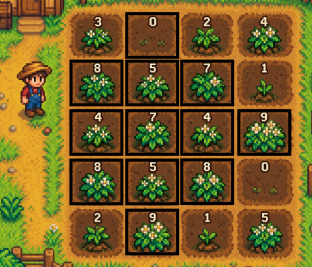
\includegraphics[scale=0.2]{fazendinha.png}
\end{center}

%- endblock

%- block editorial
This is the editorial.
%- endblock
